%%% -*- TeX-master: "../main" -*-
\chapter{Introduction}
\label{cha:introduction}

In \citeyear{dvs} \citeauthor{dvs} presented a type of image sensor that they
called an asynchronous temporal contrast vision sensor \cite{dvs} which sees the
world as a series of light intensity changes through time instead of a sequence
of still frames. Since then a spin-off company markets the chip to research
institutes around the world under the name Dynamic Vision Sensor (DVS). In this
thesis we use GRUs, short for gated recurrent units \cite{gru}, to recognize
hand gestures in DVS recordings. GRUs are a type of neural network layer for
sequence learning and a recent simplification of the influential Long Short-Term
Memory (LSTM) layer \cite{lstm}.

Computer vision has revolved around images as still frames and series of these,
also known as videos, since its inception in the late 60s when Martin Minsky at
MIT asked his undergraduate student Gerald Jay Sussman to solve vision as a
summer project. Starting in the 70s hordes of researchers have developed methods
to track objects through video, reconstruct 3D maps of the world from one or
multiple frames, recognize faces in images and much more. Nonetheless, chips
like the DVS leave all this behind and break open a new branch of vision --
neuromorphic vision.

Neuromorphic means that the DVS draws its inspiration from the way vision
happens on the retina of a biological eye, e.g. the human eye. This manifests
itself in its eponymous attributes: asynchronous and temporal contrast. The
former means that each of the DVS' pixels generates an intensity change event as
soon as it is triggered as opposed to the synchronous way in which a traditional
camera queries all pixels at once every few milliseconds. The latter refers to
the fact that a pixel is triggered when the change in light intensity at its
position exceeds a certain threshold. Taken together these properties make the
DVS' pixels comparable to retinal ganglion cells.

\begin{figure}[h]
  \centering
  \begin{subfigure}{0.4\textwidth}
    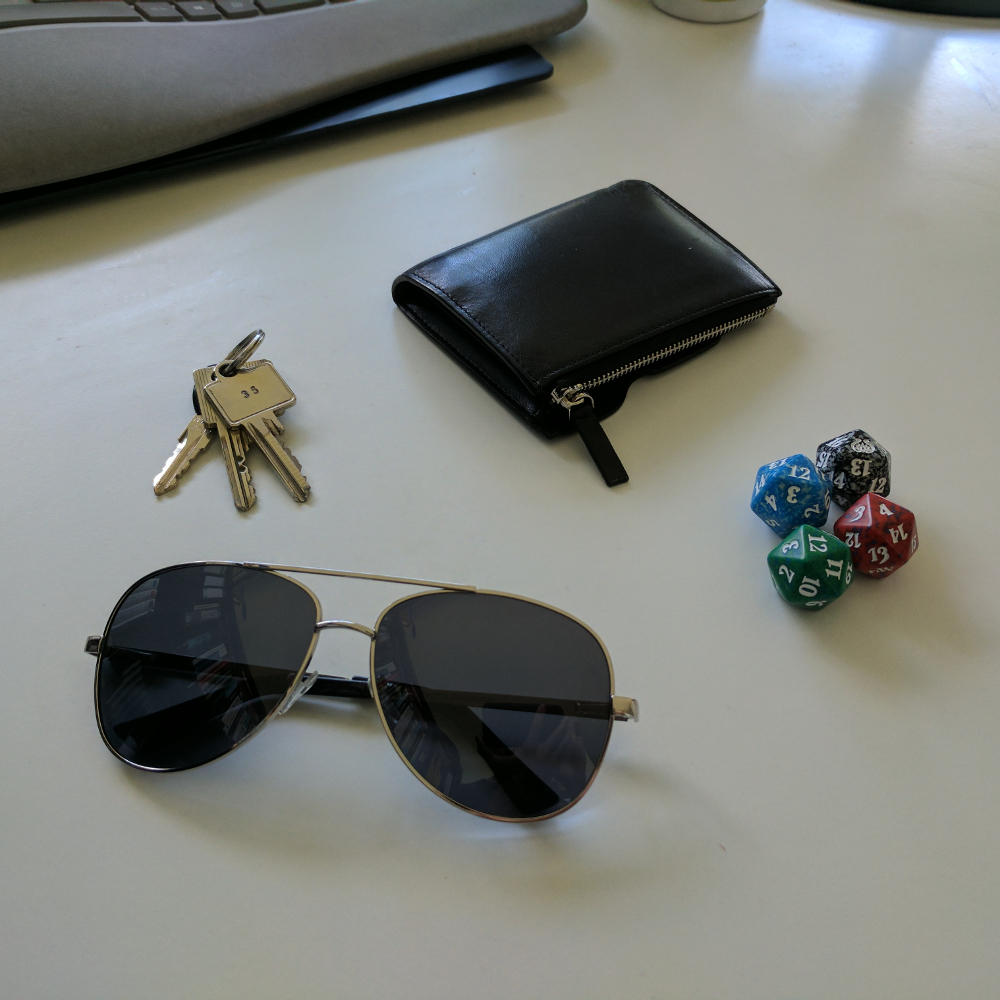
\includegraphics[width=\textwidth]{figures/introduction/objects-camera}
  \end{subfigure}
  \hspace{2em}
  \begin{subfigure}{0.4\textwidth}
    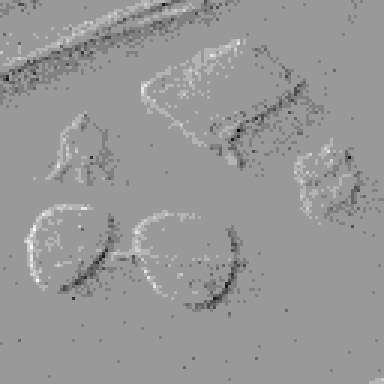
\includegraphics[width=\textwidth]{figures/introduction/objects-dvs}
  \end{subfigure}
  \caption{Keys, a wallet, dice and sunglasses captured with a camera (left) and
    with a DVS (right). The righthand picture was generated by accumulating
    events over \nicefrac{1}{30} of a second.}
\end{figure}

In recent years, deep learning has taken over the field of computer vision. It
started in \citeyear{alexnet} when \citeauthor{alexnet} blew everyone else out
of the water at the ILSVRC image classification challenge with a convolutional
neural network \cite{alexnet}. Neural networks have been refined ever since and
are now even outperforming humans in these types of tasks. The aim of this
thesis is to investigate in what capacity these successes can be transferred to
neuromorphic vision by the example of gesture recognition. The main challenges
are twofold. First, the data a DVS records is inherently temporal and each data
point on its own carries little meaning. In comparison, a video is also
temporal, yet each frame already captures a lot of the scene on its own. Equally
important is the lack of training data. The ubiquity of smartphones and cameras
has people collecting ever increasing amounts of visual data. Neuromorphic
sensors, on the contrary, are few and far between with a shortage of publicly
available data. We handle these difficulties by transforming the event stream
into fewer but richer events and recording and labeling our hand gesture
dataset.

In the next chapter, we are going to review other works regarding gesture
recognition, the DVS and deep sequence learning. Chapter \ref{cha:dvs} will
introduce the DVS in more depth and discuss its advantages over frame-based
cameras. In Chapter \ref{cha:gesture-dataset}, we describe our gesture dataset,
the process of gathering and labeling it and explore it statistically. In
Chapter \ref{cha:features} we introduce and compare three different feature
transformations to make the data more tractable for downstream methods. Chapter
\ref{cha:sequence-labeling} describes two methods for training neural networks
on sequences and how their outputs are decoded into label predictions. Chapter
\ref{cha:conclusion} concludes the thesis.
